\begin{frameExample}{Planeación de la Producción}{}
  % EXAMPLE 2.6-9 (Production Planning Problem) 
Una fábrica elabora un producto cuya unidad consta de 5 unidades de la parte A y 4 unidades de la parte B. Las dos partes A y B requieren diferentes materias primas, de las cuales están disponibles 120 unidades y 240 unidades respectivamente. Estas piezas pueden fabricarse por tres métodos diferentes. Los requisitos de materia prima por producción y el número de unidades para cada parte producida se detallan a continuación. Formule el modelo L.P. para determinar el número de corridas de producción para cada método a fin de maximizar el número total de unidades completas del producto final.

{\centering
%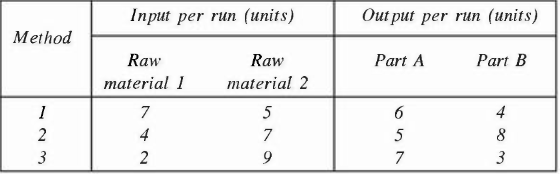
\includegraphics[scale=0.5]{example_production-planning_gupta}
  \scalebox{0.7}{%
    \begin{tabular}{ccccc}
      \toprule
  &\multicolumn{2}{c}{Entrada Por Corrida (unidades)}&\multicolumn{2}{c}{Salidas Por Corrida (unidades)}\\
  \cmidrule{2-5}
  Método&Materia & Materia & Parte&Parte \\
        &prima 1& prima 2&A&B\\
  \midrule
  1&7 &5 &6& 4\\
  2&4&7&5&8\\
  3&2&9&7&3\\
  \bottomrule
\end{tabular}
  } % \scalebox
\par}
\end{frameExample}

\begin{frameExample}{Planeación de la Producción}{}
  La función objetivo a maximizar es  \[ Z = \min \left(  \frac{6x_1 + 5x_2 + 7x_3}{5}, \frac{4x_1 + 8x_2 + 3x_3}{4}\right ) \]
  Las restricciones de disponibilidad de materias primas son:
  \begin{flalign*}
    7x_1 + 4x_2 +2x_3 &\leq 120\\
    5x_1 + 7x_2 +9x_3 &\leq 240\\
  \end{flalign*}
  La formulación anterior viola las propiedades de un programa lineal porque el objetivo es una función no lineal. El modelo se puede transformar a su versión equivalente lineal de la siguiente manera. 
  \[ y =  \min \left(  \frac{6x_1 + 5x_2 + 7x_3}{5}, \frac{4x_1 + 8x_2 + 3x_3}{4}\right )\]
  
\end{frameExample}

\begin{frameExample}{Planeación de la Producción}{}
  Tenemos entonces que
  \begin{flalign*}
    \frac{6x_1 + 5x_2 + 7x_3}{5} & \geq y\\
    \frac{4x_1 + 8x_2 + 3x_3}{4} & \geq y
  \end{flalign*}

  Por lo que el modelo matemático es:
\[ \max Z = y \]
sujeto a (s.t.)
  \begin{columns}[t]
    \column{0.4\textwidth}
\begin{flalign*}
    7x_1 + 4x_2 + 2x_3 & \leq 120\\
    5x_1 + 7x_2 + 9x_3 & \leq 240\\
  \end{flalign*}
  \column{0.4\textwidth}
    \begin{flalign*}
    6x_1 + 5x_2 + 7x_3 - 5y & \geq 0\\
    4x_1 + 8x_2 + 3x_3 - 4y & \geq 0\\
  \end{flalign*}
  \end{columns}
$x_1, x_2, x_3, y   \geq 0 $
\end{frameExample}
%%% Local Variables:
%%% mode: latex
%%% TeX-master: "../slides"
%%% End:
